% 1108.tex
% 研究型文章学习笔记模板
% 建议使用 XeLaTeX 编译(支持中文)
\documentclass[11pt,a4paper]{article}
\usepackage[margin=2.5cm]{geometry}
\usepackage{fontspec}
\usepackage{xeCJK}
\usepackage{amsmath,amssymb}
\usepackage{graphicx}
\usepackage{float}
\usepackage{caption}
\usepackage{booktabs}
\usepackage{enumitem}
\usepackage[colorlinks=true,linkcolor=blue,citecolor=blue,urlcolor=blue]{hyperref}
\usepackage{fancyhdr}
\usepackage{tcolorbox}
\usepackage{datetime}

% 字体(可按需修改)
\setmainfont{TeX Gyre Termes}
\setCJKmainfont{SimSun} % Windows 常见中文字体,视系统调整

% 页眉页脚
\pagestyle{fancy}
\fancyhf{}
% \lhead{\small 研究笔记}
\rhead{\small \PaperMeta}
\cfoot{\small \thepage}

% 元数据命令(在文档开始处填写)
\newcommand{\PaperMeta}{}
\newcommand{\PaperTitle}{}
\newcommand{\PaperAuthors}{}
\newcommand{\PaperVenue}{}
\newcommand{\PaperYear}{}
\newcommand{\PaperLink}{}

% 强调框
\newtcolorbox{highlight}{colback=yellow!10,colframe=yellow!60!black,boxrule=0.5pt}

\begin{document}

% ————— 填写元数据 —————
\renewcommand{\PaperTitle}{Observation and Modulation of the Quantum Mpemba Effect on a Superconducting Quantum Processor}
\renewcommand{\PaperAuthors}{Yueshan Xu, Cai-Ping Fang, Bing-Jie Chen, Ming-Chuan Wang}
\renewcommand{\PaperVenue}{ArXiv}
\renewcommand{\PaperYear}{2025}
\renewcommand{\PaperLink}{http://arxiv.org/abs/2508.07707}
\renewcommand{\PaperMeta}{\PaperTitle\ --- \PaperYear}

% ————— 路径设置 —————
\newcommand{\paperpath}{D:/B_Dr/arXiv-2508.07707v1/}
\graphicspath{{\paperpath}}

\begin{center}
    {\LARGE \textcolor{blue}{\PaperTitle}}\\[6pt]
    {\small \PaperAuthors \quad | \quad \PaperVenue \quad | \quad \PaperYear}\\
    {\small \url{\PaperLink}}
\end{center}

\tableofcontents
\vspace{6pt}
\hrule
\vspace{10pt}

% ————— 快速摘要 —————
\section*{快速摘要(TL;DR)}
\begin{enumerate}[leftmargin=*]
    \item 3--5 行总结核心思想、主要贡献、适用场景与效果。
    \item 一句话亮点:例如“提出了一个轻量级的...,在 X 数据集上将误差降低了 Y\%”。
\end{enumerate}

\section{背景介绍}
\begin{enumerate}[leftmargin=*]
    \item In non-equilibrium quantum many-body systems, the quantum Mpemba effect (QME) emerges as a counterintuitive phenomenon: systems exhibiting greater initial symmetry breaking restore symmetry faster than those with less.
    \item \textcolor{blue}{Three major research fields}
        \begin{itemize}
        \item The Mpemba effect, originally observed as faster freezing of hotter water than colder water under identical conditions, represents a counterintuitive non-equilibrium phenomenon with debated mechanisms.
        \item In open quantum systems interacting with an external environment through Markovian and non-Markovian processes. It is dominated by classical fluctuations, resembling the classical Mpemba effect
        \item In isolated quantum systems governed by intrinsic quantum dynamics. It is driven by intrinsic quantum fluctuations. \textcolor{blue}{In isolated quantum systems, the quantum Mpemba effect (QME) manifests as a remarkable phenomenon: subsystems with greater initial symmetry breaking restore symmetry faster under a symmetry-preserving Hamiltonian.} The type of system under the study:
        \begin{itemize}
            \item Quasiparticle framework for integrable systems that include 1D or 2D models.
            \item In chaotic systems using random and dualunitary circuits.
            \item Non-ergodic contexts, such as many-body localized (MBL) systems
            \end{itemize}
        \end{itemize}
    \item 伪代码/核心算法要点
\end{enumerate}


\section{实验方案}
\begin{enumerate}
    \item Here, we report the observation and control of QME using a superconducting processor featuring a unique fully connected, tunable-coupling architecture that enables precise modulation from short- to long-range interactions.
    \item 调控参量
        \begin{enumerate}
            \item interaction range
            \item potential engineering 
            \item initial state selection
        \end{enumerate}
\end{enumerate}

\subsection{哈密顿量}


实验系统由 16 个超导量子比特组成,采用全连接环状拓扑结构,具备可调耦合能力。系统的有效哈密顿量可写为:

\begin{equation}
H = \sum_{i < j} g_{ij} (\sigma^{+}_{i} \sigma^{-}_{j} + \sigma^{-}_{i} \sigma^{+}_{j}) + \sum_{i} h_i \sigma^{+}_{i} \sigma^{-}_{i}
\end{equation}

其中:
\begin{itemize}
    \item $g_{ij}/2\pi$ 表示量子比特 $Q_i$ 与 $Q_j$ 之间的耦合强度;
    \item $\sigma^{+}_{i}$ 和 $\sigma^{-}_{i}$ 分别为第 $i$ 个量子比特的升降算符;
    \item $h_i/2\pi$ 表示通过频率调制实现的在位势能,参考频率为 $\omega_{\text{ref}}/2\pi \approx 4.24\ \text{GHz}$。
\end{itemize}

为了区分不同耦合范围,我们将耦合强度分为两部分:
\begin{equation}
\begin{aligned}
H &= \sum_{i, j=i+1} g_N (\sigma^{+}_{i} \sigma^{-}_{j} + \sigma^{-}_{i} \sigma^{+}_{j}) \\
&\quad + \sum_{i < j, j \neq i+1} g_L (\sigma^{+}_{i} \sigma^{-}_{j} + \sigma^{-}_{i} \sigma^{+}_{j}) + \sum_{i} h_i \sigma^{+}_{i} \sigma^{-}_{i}
\end{aligned}
\end{equation}

其中:
\begin{itemize}
    \item $g_N/2\pi$ 表示最近邻(短程)耦合强度;
    \item $g_L/2\pi$ 表示长程耦合强度。
\end{itemize}

定义耦合比 $r = |g_N / g_L|$,用于量化不同相互作用区间:
\begin{itemize}
    \item $r \gg 1$:强短程耦合区间;
    \item $r \approx 1$:中间耦合区间;
    \item $r \ll 1$:弱短程耦合区间。
\end{itemize}

通过调节中心总线谐振器频率 $\Delta_{RQ}$ 和耦合器频率 $\Delta_{CQ}$ 相对于参考频率的失谐,可实现 $r$ 的连续调控。



% ————— 图1:量子处理器显微照片和耦合强度调制 —————
\section{实验装置与耦合调控}

\begin{figure}[H]
    \centering
    \includegraphics[width=0.95\textwidth]{Figure1/Figure1.pdf}
    \caption{
        \textcolor{blue}{量子处理器的显微照片和耦合强度调制。}
        (a) 超导量子处理器的光学显微照片,采用环状拓扑结构,包含16个量子比特,通过16个可调耦合器($C$)和中心总线谐振器($R$)互连。插图为谐振器中心约瑟夫森结的光学显微照片。
        (b) 实验协议的脉冲序列,通过$R$和$C$实现耦合强度的灵活调制。协议包括:在倾斜乘积态中初始化系统,使用Z脉冲将量子比特调至工作点(施加各种在位势),通过多量子比特量子态层析构建子系统$A=\{Q_1,Q_2,Q_3\}$的密度矩阵。
        (c,d) 有效耦合强度$g/2\pi$示意图,分别对应$r\approx 10$和$r\approx 1$,其中$r$为最近邻与长程耦合强度之比。线宽和颜色表示$g/2\pi$的大小。
    }
    \label{fig:device_and_coupling}
\end{figure}

\textcolor{blue}{关键参数说明:}
\begin{itemize}
    \item \textcolor{blue}{处理器架构:} 16量子比特全连接环状拓扑,每个量子比特电容耦合至最近邻耦合器,同时所有量子比特电容耦合至中心频率可调总线谐振器(4.5–6.5 GHz)
    \item \textcolor{blue}{实验选择:} 实验中选用14个相邻量子比特组成紧密连接链状阵列
    \item \textcolor{blue}{耦合调控:} 通过调节中心总线谐振器频率$\Delta_{RQ}$和耦合器频率$\Delta_{CQ}$实现不同耦合区间:
    \begin{itemize}
        \item 强短程耦合区间($r\approx 10$):$\Delta_{CQ}\approx 1.0$ GHz,$\Delta_{RQ}\approx 2.2$ GHz
        \item 中间耦合区间($r\approx 1$):$\Delta_{CQ}\approx 2.0$ GHz,$\Delta_{RQ}\approx 0.4$ GHz
    \end{itemize}
\end{itemize}

\textcolor{blue}{三种在位势:}
\begin{itemize}
    \item 无在位势:$h_i = 0$,所有量子比特调谐到相同的频率,所有量子比特"共振",能量均匀分布。\textcolor{red}{共振 ($h_i=0$):完美能量匹配 $\rightarrow$ 高效的能量传递 $\rightarrow$ 快速热化}
    \item 线性在位势:$h_i = \omega_{\text{ref}}/2\pi$,施加位置依赖的线性梯度场。\textcolor{red}{线性 ($h_i$ 线性变化):系统性失配 $\rightarrow$ 抑制热化,诱导局域化}
    \item 无序在位势:$h_i = \omega_{\text{ref}}/2\pi \cos(2\pi i t)$,每个量子比特施加随机的在位势。\textcolor{red}{非线性 ($h_i$ 随机变化):随机失配 $\rightarrow$ 破坏相干性,减缓弛豫}
\end{itemize}


\section{结论}
\begin{enumerate}
    \item In strong \textcolor{blue}{short-range} coupling regimes, EA crossovers during quenches from \textcolor{blue}{tilted Néel states} confirm the presence of QME.
    \item In \textcolor{blue}{intermediate coupling regimes}, \textcolor{red}{synchronized EA and entanglement entropy} dynamics reveal the \textcolor{blue}{suppression} of QME.
    \item QME reemerges with the introduction of \textcolor{red}{on-site linear potentials or quenches from tilted ferromagnetic states}, the latter proving robust against on-site disorder.
\end{enumerate}


\section{关键公式与推导}
Entanglement asymmetry (EA), defined as the relative entropy
\begin{equation}
\Delta S_A(t)=S\left(\rho_{A, Q}(t)\right)-S\left(\rho_A(t)\right)
\end{equation}
where $\rho_A$ is the reduced density matrix of subsystem $A$, $\rho_{A, Q}=\sum_q \Pi_q \rho_A \Pi_q$ denotes its projection onto the \textcolor{red}{conserved charge $Q_A$ eigenspaces}, and $S\left(\rho_A\right)$ is the von Neumann entropy of $\rho_A$. 

$\Delta S_A(t)$ captures the distance of $\rho_A$ from a \textcolor{red}{symmetric state $\rho_A,Q$} including contributions from non-local correlations within subsystem A that violate the symmetry.

This makes it a natural \textcolor{blue}{order parameter} for non-equilibrium dynamics, offering a fresh perspective on thermalization compared to traditional metrics like entanglement entropy.


% ————— 实验设置 —————
% \section{实验与结果}

% ————— 图2:EA测量实验协议及强短程耦合区间的EA动力学 —————
\section{短程相互作用区间的纠缠不对称性测量与QME观测}

\begin{figure}[H]
    \centering
    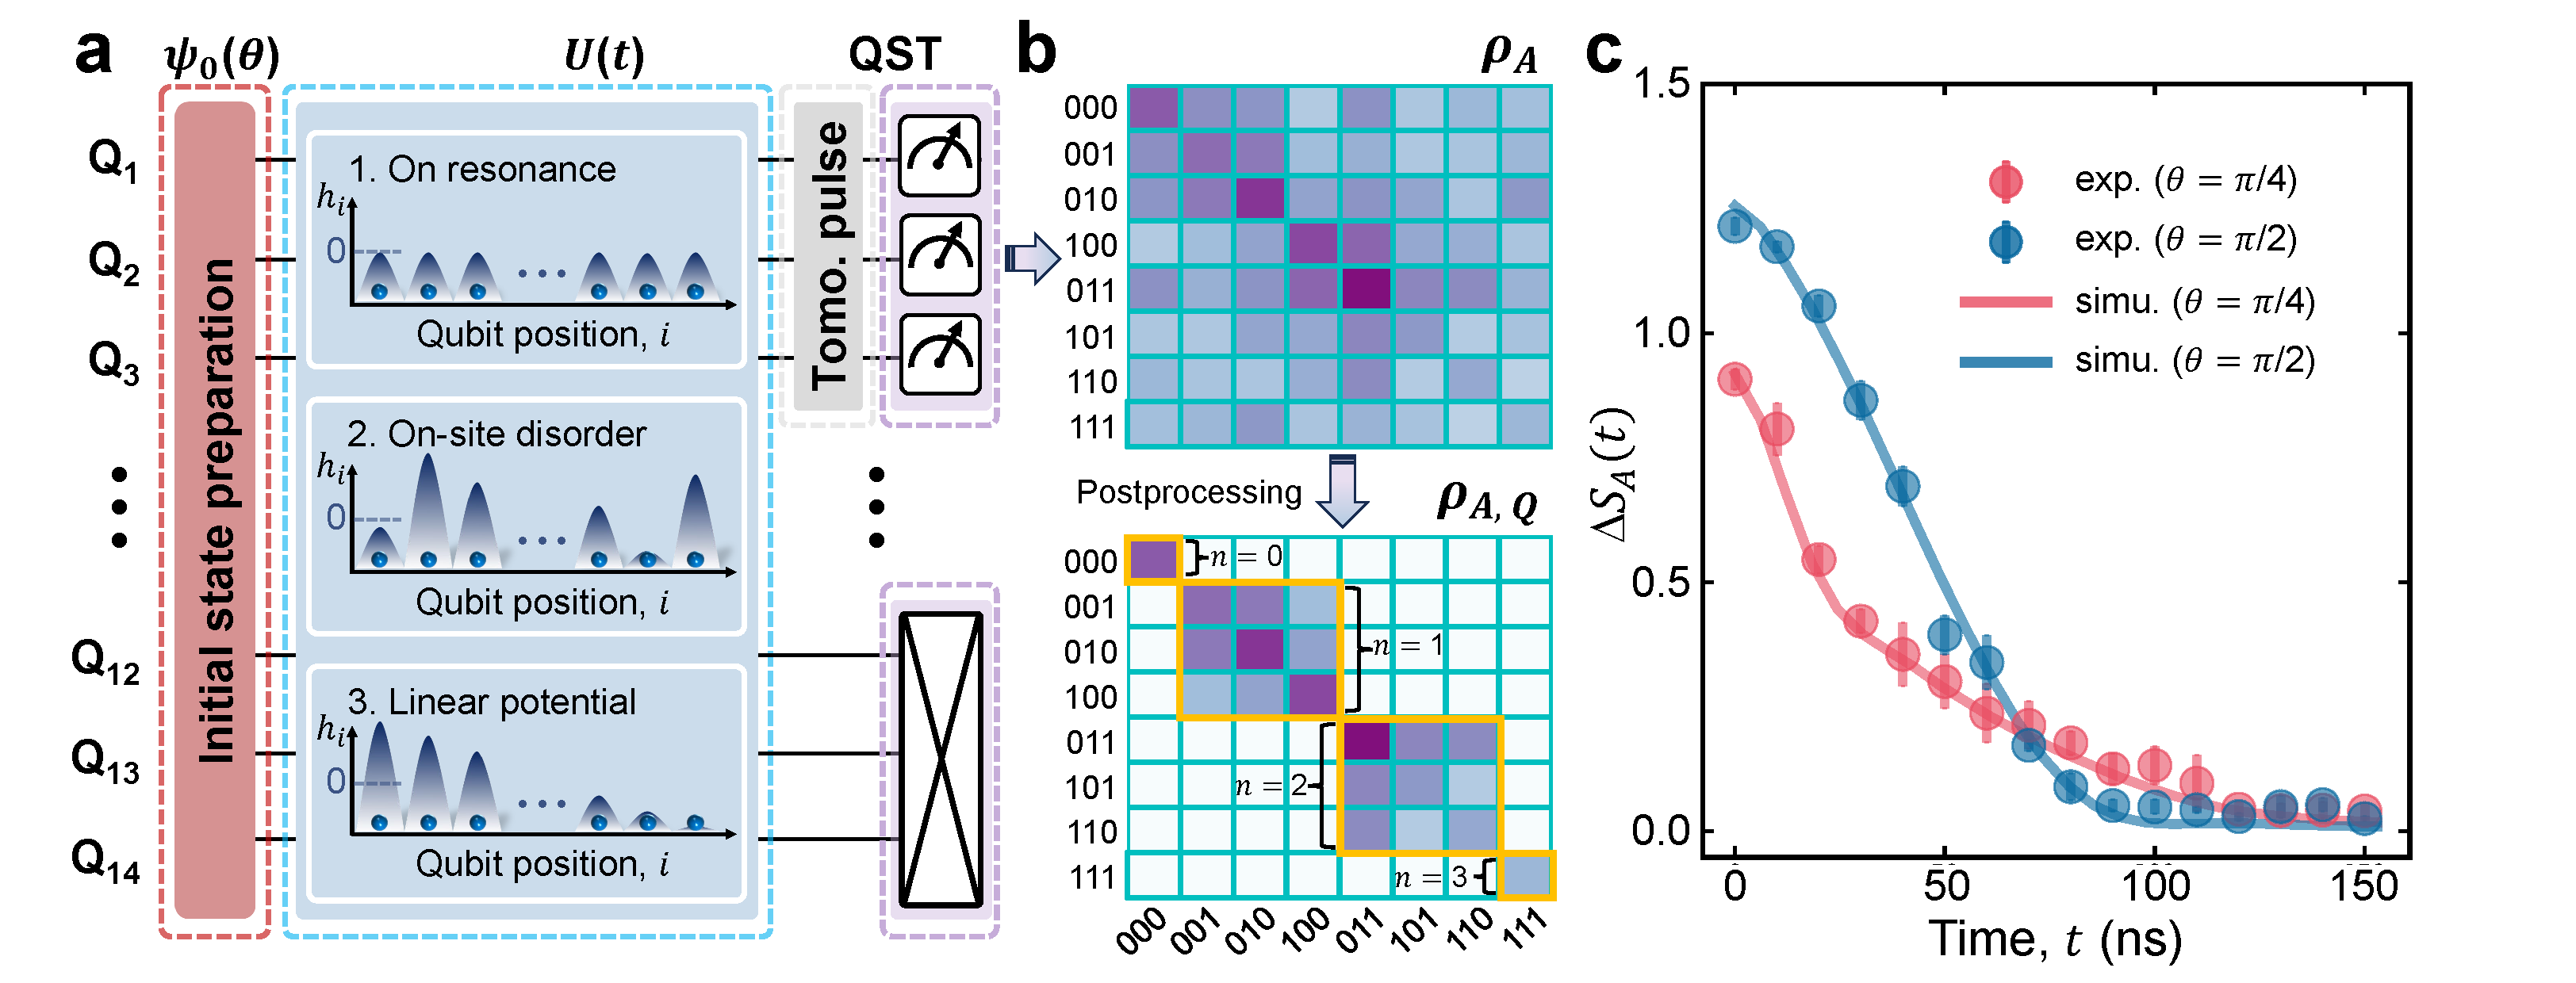
\includegraphics[width=0.95\textwidth]{Figure2/Figure2.pdf}
    \caption{
        \textcolor{blue}{强短程耦合区间($r\approx 10$)EA测量实验协议及其动力学。}
        (a) 实验协议的量子电路图。在初始态$|\Psi(\theta)\rangle$制备后,系统在工程化哈密顿量$H$下演化:$|\Psi(t)\rangle = U(t)|\Psi(\theta)\rangle = e^{-iHt}|\Psi(\theta)\rangle$,其中对量子比特施加了不同类型的在位势(共振、无序或线性梯度场)。
        (b) 通过量子态层析重建子系统$A$的密度矩阵。将密度矩阵投影到电荷算符$Q_A$的本征空间后,应用经典后处理来估计EA。
        (c) 强短程耦合区间($r\approx 10$)下量子比特共振时,倾斜Néel初始态(角度$\theta=\pi/4$和$\pi/2$)的EA动力学。观察到$\theta=\pi/2$时对称性恢复更快,并出现明显的交叉现象,证实了QME的存在。符号为实验数据,实线为包含退相干的理论结果。误差棒表示10次实验重复的标准偏差,每次包含3000次测量。
    }
    \label{fig:EA_measurement_strong_coupling}
\end{figure}

\textcolor{blue}{关于$\rho_A$和$\rho_{A, Q}$的深入理解:}
\begin{enumerate}
    \item \textcolor{blue}{约化密度矩阵 $\rho_A$}
    \begin{itemize}
        \item \textcolor{blue}{定义:} $\rho_A$ 是子系统 $A = \{Q_1, Q_2, Q_3\}$ 的约化密度矩阵,通过对总系统(14个量子比特)的密度矩阵 $\rho_{\text{total}}$ 对补集 $\bar{A} = \{Q_4, Q_5, \dots, Q_{14}\}$ 取部分迹得到:
        \begin{equation}
        \rho_A = \operatorname{Tr}_{\bar{A}} (\rho_{\text{total}})
        \end{equation}
        
        \item \textcolor{blue}{数学表示:} 在计算基下,$\rho_A$ 是一个 $8 \times 8$ 的厄米矩阵,满足:
        \begin{itemize}
            \item 半正定性:$\rho_A \succeq 0$
            \item 迹为1:$\operatorname{Tr}(\rho_A) = 1$
            \item 矩阵元 $\rho_{ij} = \langle i | \rho_A | j \rangle$,其中 $i,j \in \{000,001,\dots,111\}$
        \end{itemize}
        
        \item \textcolor{blue}{物理意义:} $\rho_A$ 完整描述了子系统 $A$ 的量子态,包含:
        \begin{itemize}
            \item 对角元:各个计算基态的概率分布
            \item 非对角元:不同基态间的量子相干性
        \end{itemize}
    \end{itemize}
    
    \item \textcolor{blue}{投影密度矩阵 $\rho_{A,Q}$}
    \begin{itemize}
        \item \textcolor{blue}{定义:} $\rho_{A,Q}$ 是 $\rho_A$ 在守恒荷 $Q_A = \sum_{i\in A} \sigma_z^i$ 的本征空间上的投影:
        \begin{equation}
        \rho_{A,Q} = \sum_{q} \Pi_q \rho_A \Pi_q
        \end{equation}
        其中 $\Pi_q$ 是投影到本征值 $q$ 对应子空间的投影算符。
        
        \item \textcolor{blue}{本征值分组:} 对于3量子比特系统,$Q_A$ 的本征值为激发数($|1\rangle$ 的个数):
        \begin{align*}
        q = 0 &: \{|000\rangle\} \quad \text{(1维)} \\
        q = 1 &: \{|001\rangle, |010\rangle, |100\rangle\} \quad \text{(3维)} \\
        q = 2 &: \{|011\rangle, |101\rangle, |110\rangle\} \quad \text{(3维)} \\
        q = 3 &: \{|111\rangle\} \quad \text{(1维)}
        \end{align*}
        
        \item \textcolor{blue}{矩阵结构:} 在计算基排序下,$\rho_{A,Q}$ 具有块对角形式:
        \begin{equation}
        \rho_{A,Q} = \begin{pmatrix}
        \text{块}_0 & 0 & 0 & 0 \\
        0 & \text{块}_1 & 0 & 0 \\
        0 & 0 & \text{块}_2 & 0 \\
        0 & 0 & 0 & \text{块}_3
        \end{pmatrix}
        \end{equation}
        其中每个块对应一个电荷子空间。
        
        \item \textcolor{blue}{物理意义:} \textcolor{red}{投影操作消除了不同电荷子空间之间的量子相干性,只保留每个电荷子空间内部的量子特性。}这使得 $\rho_{A,Q}$ 成为一个 $U(1)$ 对称的状态。
    \end{itemize}
    
    \item \textcolor{blue}{关键区别与联系}
    \begin{itemize}
        \item $\rho_A$ 可能破坏 $U(1)$ 对称性,包含不同电荷子空间间的相干项
        \item $\rho_{A,Q}$ 严格保持 $U(1)$ 对称性,不同电荷子空间间无相干性
        \item 纠缠不对称性 $\Delta S_A = S(\rho_{A,Q}) - S(\rho_A)$ 量化了对称性破缺的程度:
        \begin{itemize}
            \item $\Delta S_A = 0$:状态具有 $U(1)$ 对称性
            \item $\Delta S_A > 0$:状态破坏 $U(1)$ 对称性
        \end{itemize}
    \end{itemize}
\end{enumerate}
\textcolor{blue}{两个层面的对称性与量子Mpemba效应机制}

\subsection{对称性的两个层面}
\begin{enumerate}
    \item \textcolor{blue}{动力学对称性}:$[H, Q_A] = 0$,保证电荷守恒
    \begin{itemize}
        \item \textcolor{red}{核心关系}:算符与哈密顿量对易 $\rightarrow$ 该算符对应的物理量是守恒量,哈密顿量具有该算符生成的对称性(例如 $U(1)$ 对称性)
        \item \textcolor{blue}{数学表达}:如果 $[H, Q] = 0$,那么 $e^{-iHt} Q e^{iHt} = Q$
        \item \textcolor{blue}{深层含义}:哈密顿量在对称变换下不变,$H = U^\dagger(\phi) H U(\phi)$
    \end{itemize}

    \item \textcolor{blue}{状态对称性}:$[\rho, Q_A] = 0$,状态本身具有对称性
    \begin{itemize}
        \item \textcolor{blue}{物理意义}:状态本身具有对称性
        \item \textcolor{blue}{数学表达}:如果 $[\rho, Q] = 0$,那么 $\rho$ 在对称变换下不变,$\rho = U^\dagger(\phi) \rho U(\phi)$
        \item \textcolor{blue}{量子态特征}:状态是电荷本征态的混合或叠加,但不包含不同电荷间的相干性
    \end{itemize}
\end{enumerate}

\subsection{量子Mpemba效应的核心机制}
\begin{itemize}
    \item \textcolor{blue}{关键现象}:即使动力学是对称的($[H, Q_A] = 0$),初始状态 $\rho_A(0)$ 也可能破坏对称性,然后在演化过程中逐渐恢复对称性
    
    \item \textcolor{blue}{两种演化路径}:
    \begin{itemize}
        \item 对称的动力学 + 不对称的初始状态 $\rightarrow$ 对称性恢复过程
        \item 对称的动力学 + 对称的初始状态 $\rightarrow$ 始终保持对称性
    \end{itemize}
    
    \item \textcolor{blue}{$U(1)$ 对称性定义}:系统在绕 $z$ 轴的任意旋转下不变
\end{itemize}

\subsection{强短程耦合区间的QME机制:准粒子介导的弛豫}
\begin{itemize}
    \item \textcolor{blue}{理论基础}:在近可积的强短程耦合体系中,QME的出现可以由准粒子图像完美解释
    
    \item \textcolor{blue}{准粒子特性}:
    \begin{itemize}
        \item 可积系统存在稳定的准粒子,作为系统的集体激发
        \item 准粒子在整个演化过程中几乎不衰变
        \item 系统演化时在整个系统中产生纠缠的准粒子对
    \end{itemize}
    
    \item \textcolor{blue}{与纠缠不对称性的关系}:
    \begin{itemize}
        \item 只有子系统 $A$ 内部产生的准粒子对才对 $\Delta S_A$ 有贡献
        \item 准粒子离开子系统 $A$ 后不再贡献于内部的对称性破缺
    \end{itemize}
    
    \item \textcolor{blue}{倾斜角 $\theta$ 的关键作用}:
    \begin{itemize}
        \item \textcolor{blue}{大倾斜角 ($\theta = \pi/2$)}:初始态具有更大对称性破缺,优先激发传播速度更快的准粒子模式
        \item \textcolor{blue}{小倾斜角 ($\theta = \pi/4$)}:对称性破缺较小,激发的准粒子中慢速模式比重更高
        \item \textcolor{blue}{结果}:大倾斜角态虽然初始不对称性更强,但通过快速准粒子更快地恢复对称性,产生QME交叉现象
    \end{itemize}
\end{itemize}




\subsection{实验细节与关键发现:}
\begin{itemize}
    \item \textcolor{blue}{初始态制备:} 倾斜Néel态$|\theta\rangle_N = \bigotimes_{j=1}^{14} R_y(\theta)|s_j\rangle$,其中$|s_j\rangle = |0\rangle$($j$为奇数)或$|1\rangle$($j$为偶数)
    \item \textcolor{blue}{对称性破缺程度:} 倾斜角$\theta$控制全局$U(1)$对称性破缺程度:
    \begin{itemize}
        \item $\theta=0$或$\pi$:所有自旋沿$\sigma_z$方向排列(完全对称)
        \item $\theta=\pi/2$:所有自旋沿$\sigma_x$方向排列(最大对称性破缺)
    \end{itemize}
    \item \textcolor{blue}{耦合参数:} 
    \begin{itemize}
        \item 最近邻耦合:$g_N/2\pi = -5$ MHz
        \item 长程耦合:$g_L/2\pi \approx 0.5$ MHz
        \item 耦合比:$r \approx 10$
    \end{itemize}
    \item \textcolor{blue}{QME特征:} 虽然$|\theta=\pi/2\rangle_N$的初始EA高于$|\theta=\pi/4\rangle_N$,但其更快的对称性恢复导致更快的衰减率,产生明显的交叉现象
    \item \textcolor{blue}{物理机制:} 源于准粒子介导的弛豫,较大倾斜角$\theta$优先激发传播更快的模式,从而加速对称性恢复
\end{itemize}

\subsection{纠缠不对称性定义:}
\begin{equation}
\Delta S_A(t) = S(\rho_{A,Q}(t)) - S(\rho_A(t))
\end{equation}
其中:
\begin{itemize}
    \item $\rho_A$:子系统$A$的约化密度矩阵
    \item $\rho_{A,Q} = \sum_q \Pi_q \rho_A \Pi_q$:在守恒荷$Q_A$本征空间上的投影
    \item $S(\rho)$:冯·诺依曼熵
\end{itemize}


\section{QME在中间耦合区间的抑制}
Investigate the sensitivity of QME to \textcolor{red}{thermalization processes.}

\subsection{辨析可积与热化}
\begin{enumerate}
\item 可积$\rightarrow$不可热化
\item 不可积+无局域化$\rightarrow$通常可以热化(满足本征态热化假设ETH)
\item 不可积 + 强无序 $\rightarrow$ 可能多体局域化MBL(不热化)(有无穷多个局域守恒量,满足的是面积律,保持初态记忆)(强无序破坏共振条件,能量不匹配抑制跃迁)
\end{enumerate}


\subsection{实验设置与参数}
\begin{itemize}
    \item \textcolor{blue}{耦合区间}:中间耦合区间($r \approx 1$)
    \item \textcolor{blue}{耦合参数}:
    \begin{itemize}
        \item 最近邻耦合:$g_N/2\pi = -2$ MHz
        \item 长程耦合:$g_L/2\pi \approx -2$ MHz
        \item 耦合比:$r = |g_N/g_L| \approx 1$
    \end{itemize}
    \item \textcolor{blue}{在位势}:共振条件(所有量子比特调至$\omega_{\text{ref}}/2\pi \approx 4.24$ GHz)
    \item \textcolor{blue}{初始态}:与强短程耦合区间相同的倾斜Néel态($\theta = \pi/4$和$\pi/2$)
\end{itemize}

\subsection{关键实验结果}
\begin{figure}[H]
    \centering
    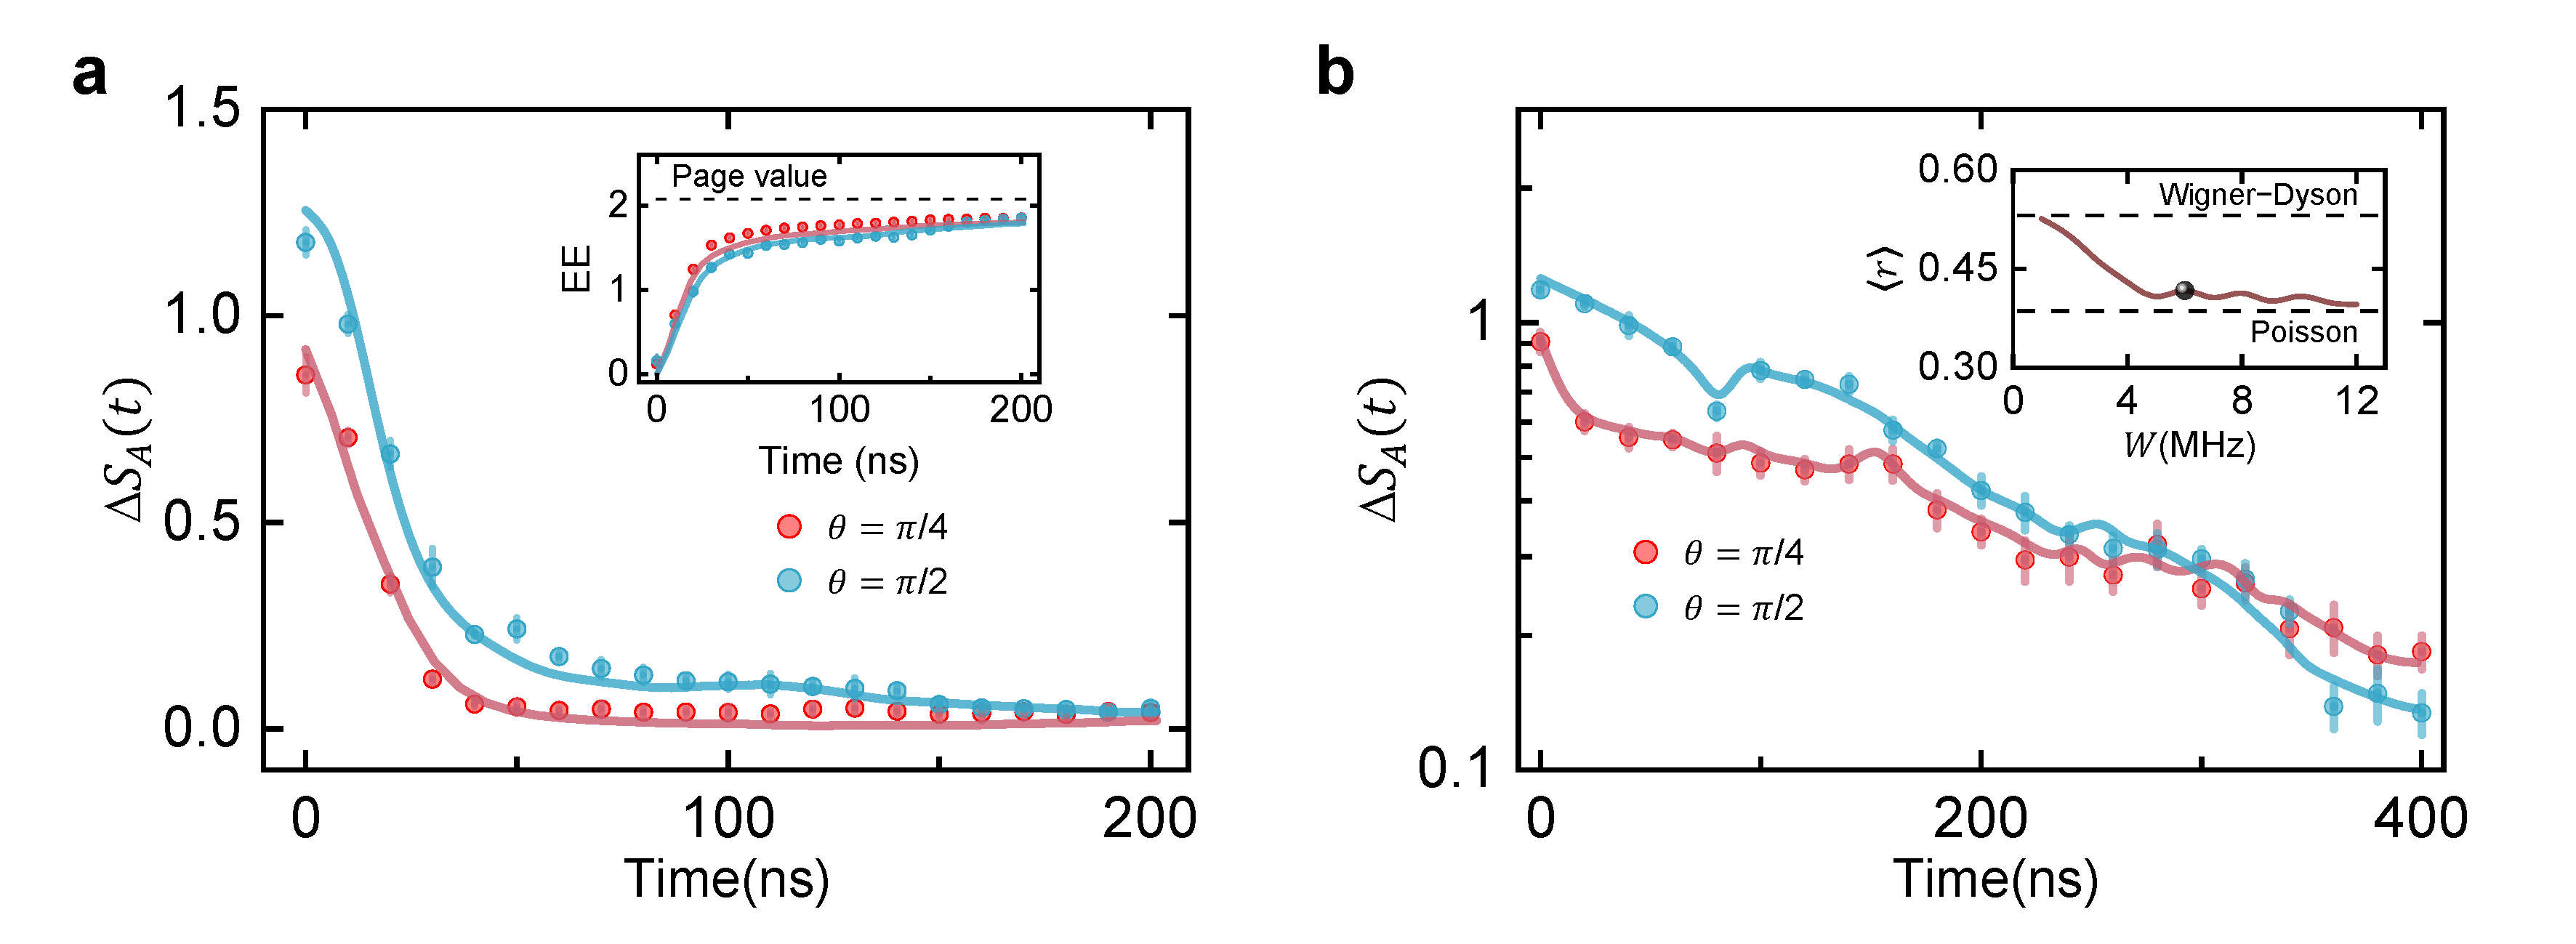
\includegraphics[width=0.95\textwidth]{Figure3/Figure3.pdf}
    \caption{
        \textcolor{blue}{中间耦合区间($r \approx 1$)的EA动力学。}
        (a) 共振条件下倾斜Néel态的EA动力学,显示$\theta = \pi/2$的态对称性恢复更慢,导致QME抑制。
        插图为纠缠熵动力学,显示两个态都趋于Page值,表明系统热化。
        (b) 引入线性势($W = 6$ MHz)后EA动力学,显示QME重新出现。
        插图为平均能级间距比$\langle r \rangle$随$W$的变化,表明系统从热化相向局域化相转变。
    }
    \label{fig:intermediate_coupling}
\end{figure}

\textcolor{blue}{图~\ref{fig:intermediate_coupling}(a)}的主图和插图都是红色线更快,说明对称性恢复的速度与热化速度成正相关。插图的红蓝线刚开始都是呈现线性增长。主图刚开始呈现线性下降。\textcolor{magenta}{EA与EE配合说明,相互验证。}


\textcolor{blue}{关于热化:}
热吉布斯系综是描述系统在热平衡状态下的统计分布。

\textcolor{blue}{关于Page value:}
根据ETH,非可积量子系统的子系统behaves like一个随机态,纠缠熵趋于一个Page value。

\textcolor{red}{Page value:}一个随机纯态中,子系统的纠缠熵的平均值。

\begin{equation}
\left\langle S_A\right\rangle_{\mathrm{Page}} \approx \ln (2) \times \min \left(N_A, N_B\right)-\frac{1}{2} \times \frac{2^{\min \left(N_A, N_B\right)}}{2^{\max \left(N_A, N_B\right)}}
\end{equation}

对于本文的总系统$N=14$,子系统$A=3$,剩余系统$B=11$,$\min \left(N_A, N_B\right) = 3$,$\max \left(N_A, N_B\right) = 11$。

因此,Page value为:
\begin{equation}
\left\langle S_A\right\rangle_{\mathrm{Page}} \approx \ln (2) \times 3-\frac{1}{2} \times \frac{2^{3}}{2^{11}} \approx 2.08
\end{equation}

类似于经典热力学由温度确定的平衡态,量子多体系统由Page value确定纠缠熵。


\textcolor{blue}{主要观测现象:}
\begin{itemize}
    \item \textcolor{blue}{QME抑制}:在中间耦合区间,更大的初始对称性破缺($\theta = \pi/2$)导致\textcolor{blue}{更慢}的对称性恢复
    \item \textcolor{blue}{无动力学交叉}:EA曲线单调衰减,没有出现强短程耦合区间中的交叉现象
    \item \textcolor{blue}{热化特征}:纠缠熵线性增长并趋于Page值,表明系统达到热平衡
\end{itemize}

\subsection{物理机制解释}
\begin{itemize}
    \item \textcolor{blue}{热化主导}:中间耦合强度破坏了系统的可积性,使动力学由热化过程主导
    \item \textcolor{blue}{对称性恢复与热化的关联}:对称性恢复速率与热化速率正相关
    \item \textcolor{blue}{倾斜角效应}:较小倾斜角($\theta = \pi/4$)的态热化更快,因此对称性恢复也更快
    \item \textcolor{blue}{与强短程耦合的对比}:在可积性主导的强短程耦合中,准粒子机制导致反常动力学;在热化主导的中间耦合中,系统遵循正常的热化行为
\end{itemize}

\subsection{理论验证}
通过计算纠缠熵动力学验证热化假设:
\begin{itemize}
    \item 两个初始态的EE都增长并接近Page值
    \item EE的演化与EA动力学密切相关
    \item 较小倾斜角的态表现出更快的EE增长,对应更快的热化速率
\end{itemize}

\subsection{重要意义}
\begin{itemize}
    \item 首次实验展示了通过调节耦合强度可以实现QME的\textcolor{blue}{可控抑制}
    \item 阐明了对称性恢复与热化过程之间的\textcolor{blue}{内在联系}
    \item 为理解量子多体系统中非平衡动力学提供了重要见解
    \item 展示了超导量子处理器在研究多体物理中的强大能力
\end{itemize}

\textcolor{blue}{核心结论:}在中间耦合区间,热化过程主导系统动力学,导致QME被抑制。这表明QME的出现强烈依赖于系统的可积性和热化性质,为理解量子多体非平衡动力学提供了重要线索。




% ————— 个人笔记与 TODO —————
\section{个人笔记 }
\textcolor{blue}{什么是本征?}
“本征”这个词源于德语“eigen”,意思是“自己的”、“固有的”、“特征的”。
\textcolor{red}{本征方程}是指一个线性算子作用在本征态上时,其结果等于\textcolor{red}{本征值}乘以\textcolor{red}{本征态}本身。形式上,设$\hat{A}$是一个线性算子,$| \psi \rangle$是$\hat{A}$的本征向量,$\lambda$是$\hat{A}$在$| \psi \rangle$上的本征值,则有:
\begin{equation}
\hat{A} | \psi \rangle = \lambda | \psi \rangle
\end{equation}

\textcolor{red}{物理意义:}
如果一个系统处于算符 $\hat{A}$ 的某个本征态上,那么你测量这个物理量 $\hat{A}$ 时,会得到一个确定无疑的结果,这个结果就是对应的本征值。

\vfill
{\small 记录时间:\today\ \currenttime}

\end{document}